\documentclass[11pt]{article}
\usepackage[margin=1in]{geometry}
\usepackage{amsmath,amssymb,amsthm}
\usepackage{graphicx}
\usepackage[hidelinks]{hyperref}

\newtheorem{theorem}{Theorem}
\newtheorem{remark}{Remark}

\DeclareMathOperator{\ran}{ran}
\newcommand{\R}{\mathbb R}
\newcommand{\N}{\mathbb N}
\newcommand{\C}{\mathbb C}
\newcommand{\cB}{\mathcal B}
\newcommand{\cW}{\mathcal W}

\title{Spectral-rich sharpness for a second-order semigroup approximation estimate}
\author{FA/Banach run packet for arXiv:1801.06749}
\date{2026-07-18}

\begin{document}
\maketitle

\section*{Source problem}

The source paper is A. Gomilko, S. Kosowicz, and Yu. Tomilov,
\emph{A general approach to approximation theory of operator semigroups},
arXiv:1801.06749, published in \emph{Journal de Mathematiques Pures et
Appliquees} 127 (2019), 216--267.

Corollary 4.10 of the source paper states that, if \(-A\) generates a bounded
\(C_0\)-semigroup on \(X\), \((g_t)_{t>0}\subset \cB_4\), and
\(M=\sup_{t\geq 0}\|e^{-tA}\|\), then for all \(t>0\), \(n\in\N\), and
\(x\in\operatorname{dom}(A^3)\),
\[
 \|g_t^n(tA/n)x-e^{-tA}x-(2n)^{-1}(g_t''(0)-1)t^2e^{-tA}A^2x\|
 \leq M C(g_t)t^3n^{-3/2}\|A^3x\|.
\]
After proving sharpness only for a shift semigroup on \(C_0(\R)\) and Euler's
formula, the authors state that the optimality of this estimate should hold in
a more general context.

\begin{center}
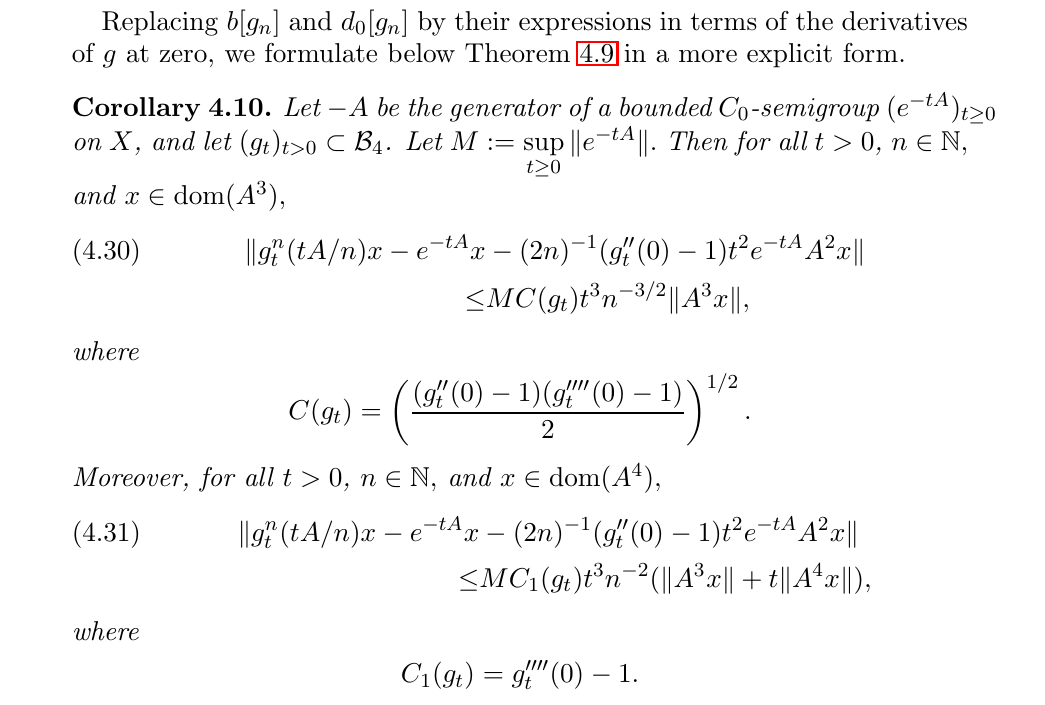
\includegraphics[width=0.95\linewidth]{figures/corollary_4_10_crop.png}
\end{center}

\begin{center}

\includegraphics[width=0.95\linewidth]{figures/open_problem_crop.png}
\end{center}

This packet proves such a general-context sharpness result under the same
spectral-rich hypothesis used in Proposition 4.11 of the source paper.  The
result is partial because it treats a fixed \(g\) and a natural spectral class,
not all possible bounded semigroups or all varying families \((g_t)\).

\section*{Idea of the proof}

The source proof of first-order optimality tests the HP functional calculus on
large imaginary spectral points of size \(\sqrt n/t\).  The same test is
exactly tuned to the second-order remainder.  Along
\(z_n=\pm i\sqrt n\), Taylor expansion gives
\[
 n\log g(z_n/n)=-z_n-a[g]+O(n^{-1/2}),
\]
because \(z_n^2/n=-1\).  After subtracting the second-order correction, the
scalar remainder tends to \(e^{-a[g]}-1+a[g]\), which is positive whenever
\(g\neq e^{-z}\).  Spectral mapping then transfers this nonzero scalar
boundary value into an operator-norm lower bound of order \(t^3n^{-3/2}\).

\section*{Notation}

For \(g\in\cB_2\) put
\[
  a[g]=\frac{g''(0)-1}{2}.
\]
The source paper observes that \(a[g]\geq 0\), and that \(a[g]=0\) if and only
if \(g(z)\equiv e^{-z}\).  For fixed \(g\in\cB_4\) define the scalar
second-order remainder
\[
  q_{t,n}(z)=g^n(tz/n)-e^{-tz}-a[g]\,n^{-1}t^2z^2e^{-tz}.
\]
The regularized remainder multiplier is
\[
  h_{t,n}(z)=z^{-3}q_{t,n}(z),
\]
with the removable value at \(z=0\).  This is the HP-calculus multiplier
corresponding to \(A^{-3}\) times the second-order remainder, understood in
the same extended-calculus sense used in Proposition 4.11 of the source paper.

\section*{Main result}

\begin{theorem}
Let \(-A\) be the generator of a bounded \(C_0\)-semigroup on a Banach space
\(X\), and assume \(\overline{\ran(A)}=X\).  Suppose that
\[
  \{\,|s|:\ s\in\R,\ is\in\sigma(A)\,\}=\R_+ .
\]
Let \(g\in\cB_4\) and \(g(z)\not\equiv e^{-z}\).  Then for every \(t>0\),
\[
 \liminf_{n\to\infty} n^{3/2}t^{-3}\,\|h_{t,n}(A)\|
 \geq e^{-a[g]}-1+a[g] >0 .
\]
Consequently, in this spectral-rich class the \(t^3n^{-3/2}\) rate in
Corollary 4.10 cannot be replaced by \(o(t^3n^{-3/2})\) for the regularized
third-order norm of the second-order remainder.
\end{theorem}

\begin{proof}
Set \(a=a[g]\).  Since \(g\neq e^{-z}\), the moment identity for functions in
\(\cB_2\) gives \(a>0\).  By the definition of \(\cB_4\), the boundary Taylor
expansion at the origin is
\[
  g(w)=1-w+\frac{g''(0)}2w^2+O(|w|^3).
\]
For all sufficiently small \(w\), \(g(w)\) is nonzero and hence
\[
  \log g(w)=-w+a w^2+O(|w|^3).
\]

Fix \(t>0\).  By the spectral hypothesis, for each \(n\) we may choose
\(\varepsilon_n\in\{-1,1\}\) such that
\[
  \lambda_n=\varepsilon_n i\sqrt n/t\in\sigma(A).
\]
Put \(z_n=t\lambda_n=\varepsilon_n i\sqrt n\) and \(w_n=z_n/n\).  Then
\[
 n\log g(w_n)
 =-z_n+a\frac{z_n^2}{n}+O(n|w_n|^3)
 =-z_n-a+O(n^{-1/2}),
\]
because \(z_n^2/n=-1\).  Hence
\[
  g^n(z_n/n)=e^{-z_n}\big(e^{-a}+O(n^{-1/2})\big).
\]
Therefore
\[
\begin{aligned}
 q_{t,n}(\lambda_n)
 &=g^n(z_n/n)-e^{-z_n}-a\,n^{-1}z_n^2e^{-z_n}\\
 &=e^{-z_n}\big(e^{-a}-1+a+O(n^{-1/2})\big).
\end{aligned}
\]
Since \(|e^{-z_n}|=1\), it follows that
\[
  |q_{t,n}(\lambda_n)|\longrightarrow e^{-a}-1+a .
\]

The scalar function \(h_{t,n}\) belongs to the HP algebra after removing the
singularity at the origin: the numerator has vanishing Taylor coefficients
through order two, and the integral representation behind Corollary 4.10
gives the corresponding bounded HP multiplier.  Applying the spectral mapping
theorem for the HP calculus, as in Proposition 4.11 of the source paper, gives
\[
  \|h_{t,n}(A)\|
  \geq r(h_{t,n}(A))
  \geq |h_{t,n}(\lambda_n)|.
\]
But \(|\lambda_n|^{-3}=t^3n^{-3/2}\), so
\[
  n^{3/2}t^{-3}|h_{t,n}(\lambda_n)|
  =|q_{t,n}(\lambda_n)|
  \longrightarrow e^{-a}-1+a .
\]
The displayed lower bound follows.  Finally \(e^{-a}-1+a>0\) for every
\(a>0\), completing the proof.
\end{proof}

\section*{Verifier report}

The proof is analytic.  As a sanity check, the script
\texttt{code/scalar\_asymptotic\_check.py} evaluates the scalar residual for
Euler's formula \(g(z)=(1+z)^{-1}\), where \(a[g]=1/2\), along
\(z_n=i\sqrt n\).  The output converges to
\(e^{-1/2}-1+1/2\), as predicted by the proof.

\section*{Limitations and novelty status}

This is not a full theorem for arbitrary bounded \(C_0\)-semigroups.  It proves
optimality for the spectral-rich class
\(\{|s|:is\in\sigma(A)\}=\R_+\), the same kind of hypothesis used by the source
paper for first-order optimality.  Concrete examples are available, for
instance multiplication generators with spectrum \(i\R\) on \(L^2(\R)\).

Before promotion, the run indexes were searched for arXiv:1801.06749, the
label \texttt{RowA0++}, and close phrases involving second-order semigroup
optimality and \(n^{-3/2}\).  Web searches on 2026-07-18 for the exact title,
the deferred-general-argument phrase, and close scalar-remainder phrases found
the source paper and mirrors but no later exact answer.  Novelty confidence is
therefore moderate-high, subject to human review.

\section*{Human-review recommendation}

Review the HP-calculus regularization line in the proof: the scalar asymptotic
and spectral choice are straightforward, and the only technical point is that
the regularized multiplier \(h_{t,n}\) is legitimate in the same functional
calculus setting as Proposition 4.11.  If accepted, this packet supplies the
general optimality argument that the source paper deferred for Corollary 4.10
within the natural spectral-rich class.

\begin{thebibliography}{9}

\bibitem{GKT}
A. Gomilko, S. Kosowicz, and Yu. Tomilov,
\emph{A general approach to approximation theory of operator semigroups},
Journal de Mathematiques Pures et Appliquees 127 (2019), 216--267.
arXiv:1801.06749.

\end{thebibliography}

\end{document}
